\documentclass[a4paper]{report}
\usepackage[utf8]{inputenc}
\usepackage[portuguese]{babel}
\usepackage{hyperref}
\usepackage{a4wide}
\hypersetup{pdftitle={TP2:  Protocolo IPv4  (Parte I)},
pdfauthor={João Teixeira, José Ferreira, Miguel Solino},
colorlinks=true,
urlcolor=blue,
linkcolor=black}
\usepackage{subcaption}
\usepackage[cache=false]{minted}
\usepackage{listings}
\usepackage{booktabs}
\usepackage{multirow}
\usepackage{appendix}
\usepackage{tikz}
\usepackage{authblk}
\usepackage{bashful}
\usepackage{verbatim}
\usepackage{amsmath}
\usetikzlibrary{positioning,automata,decorations.markings}

\begin{document}

\title{TP2:  Protocolo IPv4  (Parte I)\\ 
\large Grupo Nº 7}
\author{João Teixeira (A85504) \and José Ferreira (A83683) \and Miguel Solino (A86435)}

\date{\today}

\begin{center}
    \begin{minipage}{0.75\linewidth}
        \centering
        
\includegraphics[width=0.4\textwidth]{images/eng.jpeg}\par\vspace{1cm}
        \vspace{1cm}
        \href{https://www.uminho.pt/PT}
        {\color{black}{\scshape\LARGE Universidade do Minho}} \par
        \vspace{1cm}
        \href{https://www.di.uminho.pt/}
        {\color{black}{\scshape\Large Departamento de Informática}} \par
        \maketitle
    \end{minipage}
\end{center}

\tableofcontents

\pagebreak
\chapter{Parte 1}
\section{Exercício 1}

\begin{figure}[H]
    \centering 
    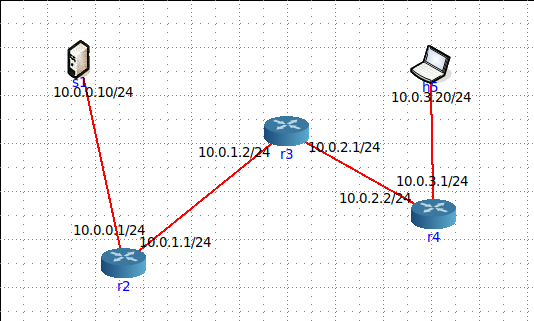
\includegraphics[width=\textwidth]{images/coreEx1.png}  
    \caption{Ex. 1 - Core}
    \label{fig:coreEx1}
\end{figure}

\begin{figure}[H]
    \centering 
    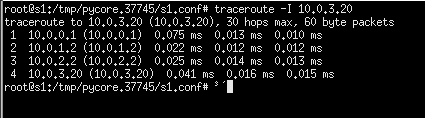
\includegraphics[width=\textwidth]{images/traceroutEx1.png}  
    \caption{Ex. 1 - Traceroute}
    \label{fig:traceroutEx1}
\end{figure}

\begin{figure}[H]
    \centering 
    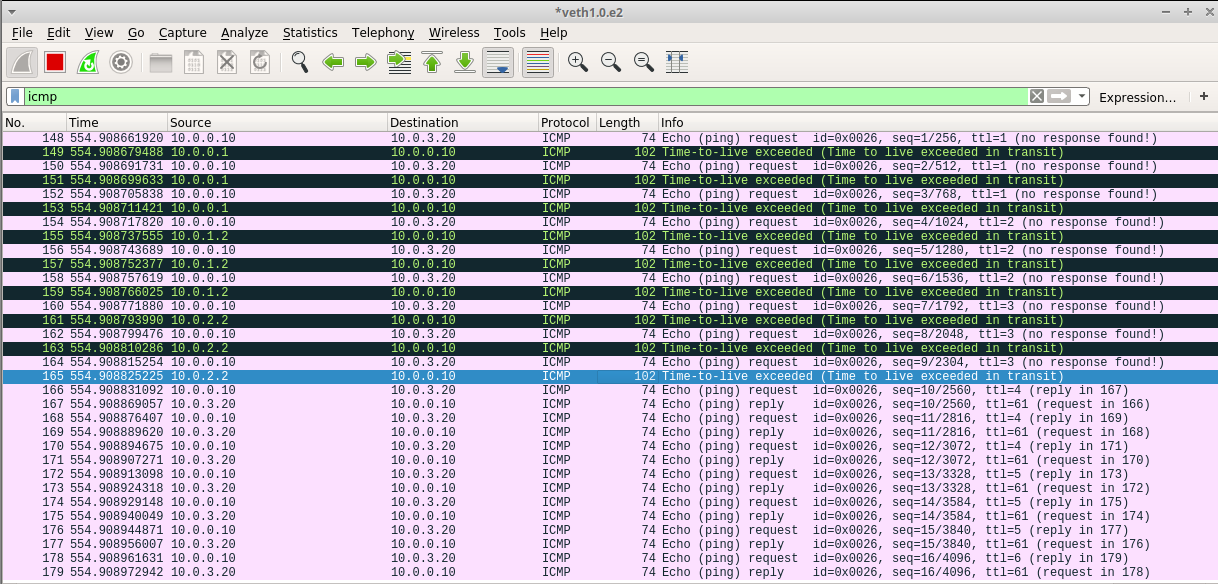
\includegraphics[width=\textwidth]{images/wiresharkEx1.png}  
    \caption{Ex. 1 - Wireshark}
    \label{fig:wiresharkEx1}
\end{figure}

\pagebreak
\section{Exercício 2}

\begin{figure}[H]
    \centering 
    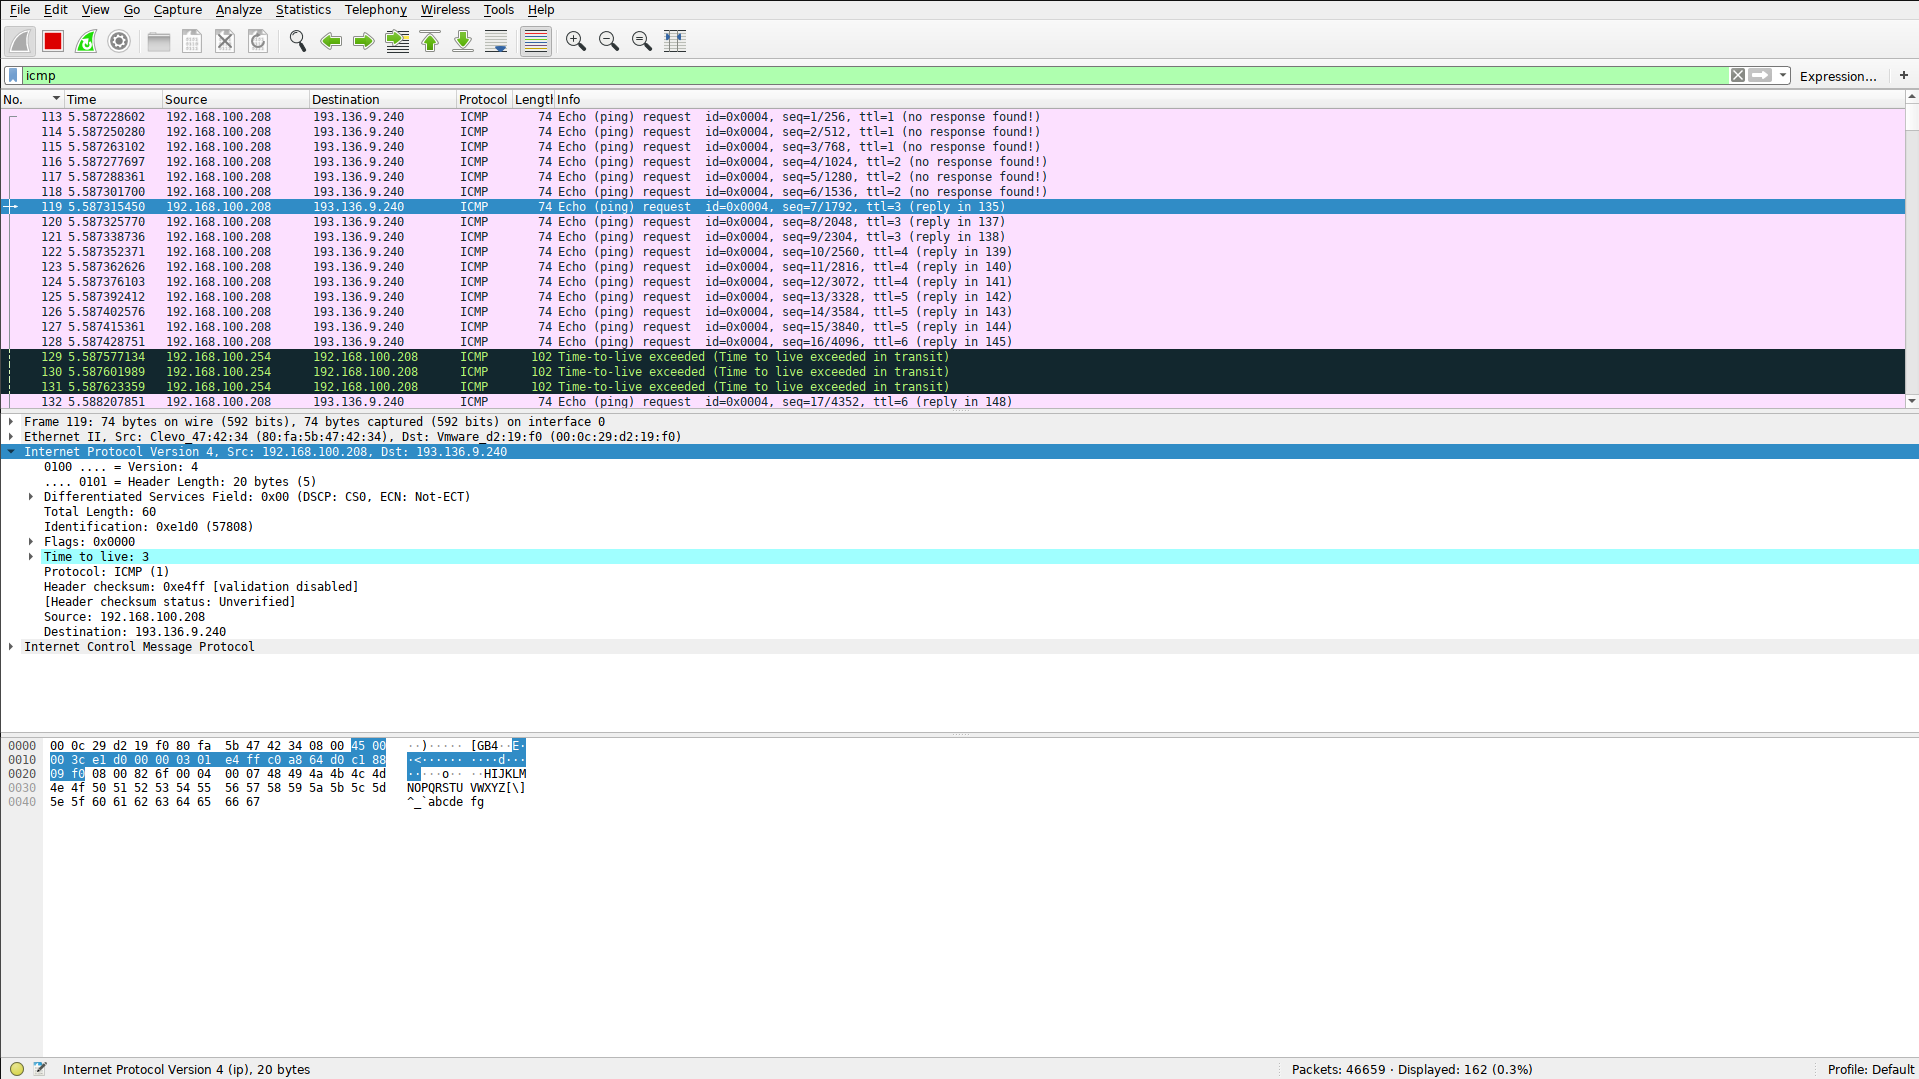
\includegraphics[width=\textwidth]{images/wiresharkEx2.png}  
    \caption{Ex. 2 - Wireshark}
    \label{fig:wiresharkEx2}
\end{figure}

\begin{figure}[H]
    \centering 
    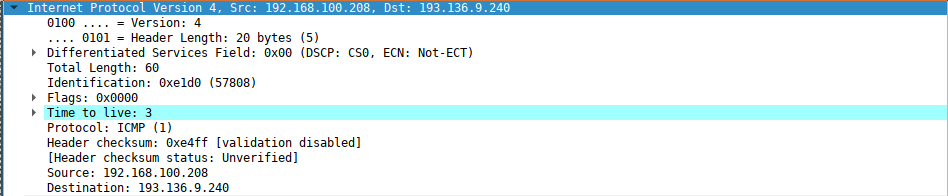
\includegraphics[width=\textwidth]{images/ipEx2.png}
    \caption{Ex. 2 - Cabeçalho IP}
    \label{fig:ipEx2}
\end{figure}

\begin{figure}[H]
    \centering 
    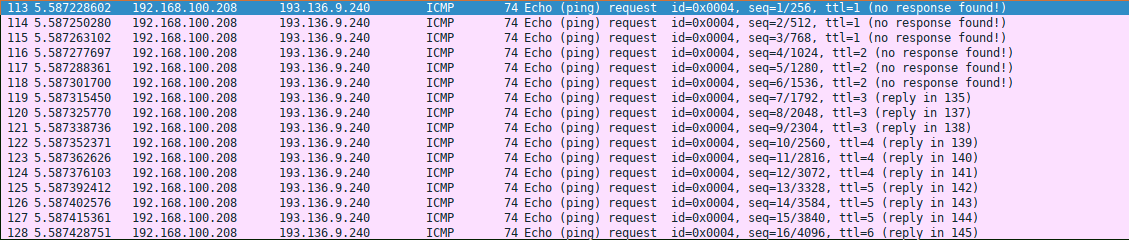
\includegraphics[width=\textwidth]{images/wiresharkSourceEx2.png}
    \caption{Ex. 2 - Tráfego Wireshark ordenado por endereço fonte}
    \label{fig:wiresharkSourceEx2}
\end{figure}

\begin{figure}[H]
    \centering 
    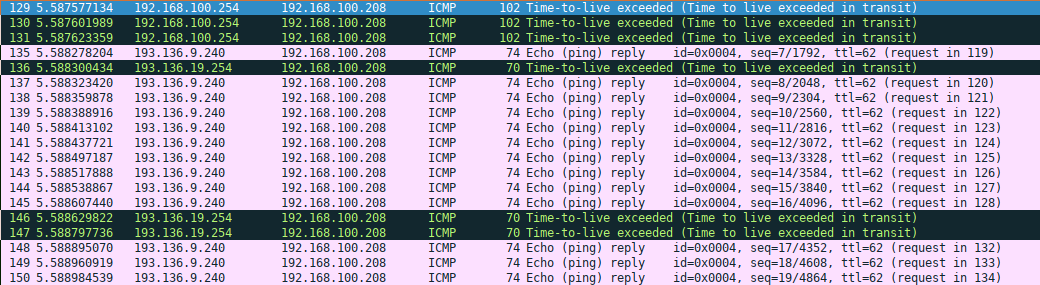
\includegraphics[width=\textwidth]{images/wiresharkDestinyEx2.png}
    \caption{Ex. 2 - Tráfego Wireshark ordenado por endereço de destino}
    \label{fig:wiresharkDestinyEx2}
\end{figure}

\pagebreak
\section{Exercício 3}

\begin{figure}[H]
    \centering 
    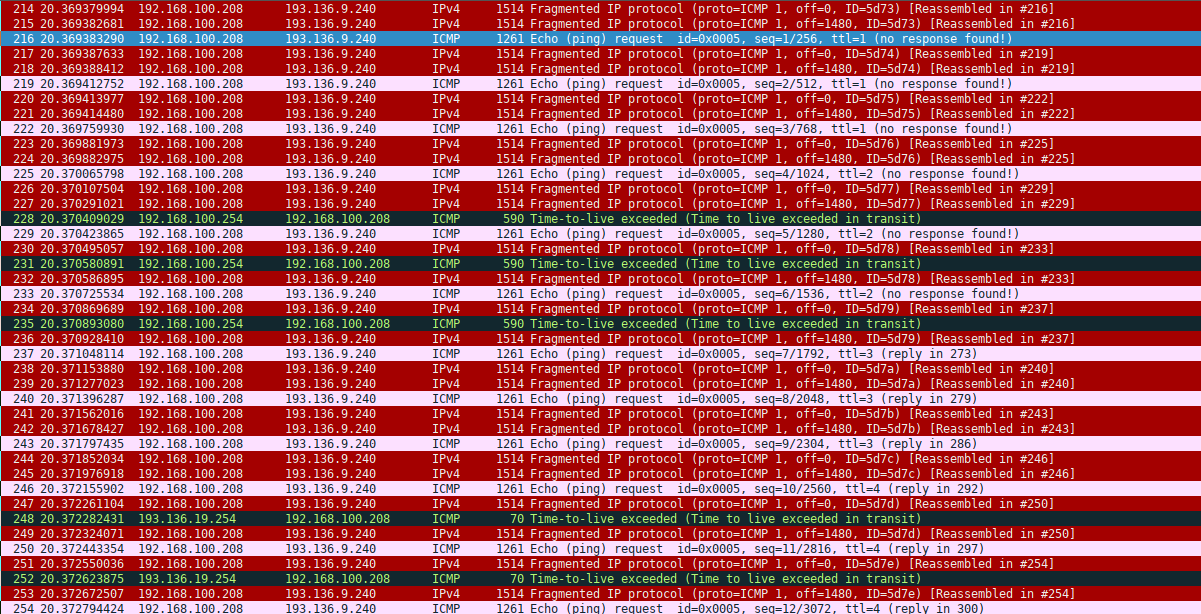
\includegraphics[width=\textwidth]{images/datagramaIpEx3.png}
    \caption{Ex.3 - Fragmentos do datagrama IP}
    \label{fig:datagramaIpEx3}
\end{figure}

\begin{figure}[H]
    \centering 
    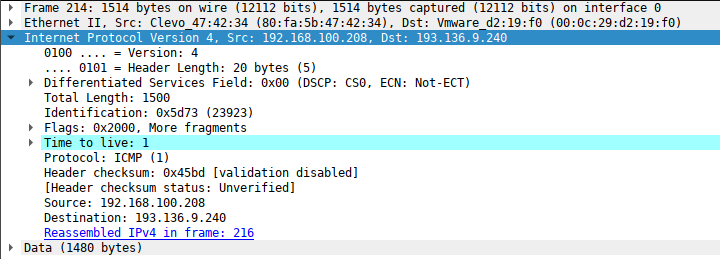
\includegraphics[width=\textwidth]{images/fragmentDatagramaIpEx3.png}
    \caption{Ex.3 - Cabeçalho do primeiro fragmento do datagrama IP}
    \label{fig:fragmentDatagramaIpEx3}
\end{figure}

\begin{figure}[H]
    \centering 
    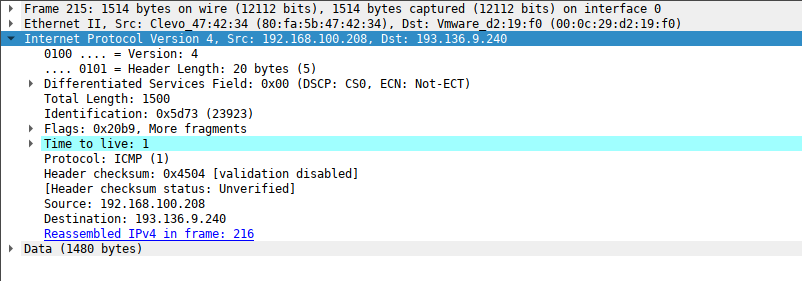
\includegraphics[width=\textwidth]{images/fragment2DatagramaIpEx3.png}
    \caption{Ex.3 - Cabeçalho do segundo fragmento do datagrama IP}
    \label{fig:fragment2DatagramaIpEx3}
\end{figure}

\chapter{Parte 2}

\begin{figure}[H]
    \centering 
    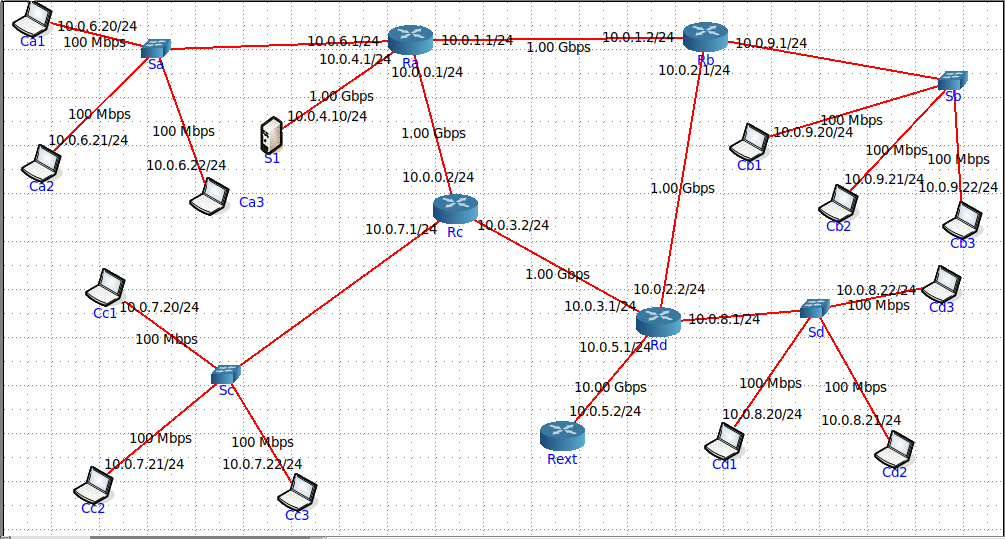
\includegraphics[width=\textwidth]{images/topologiaCore.png}
    \caption{Topologia Core}
    \label{fig:topologiaCore}
\end{figure}

\section{Exercício 1}

\begin{figure}[H]
    \centering 
    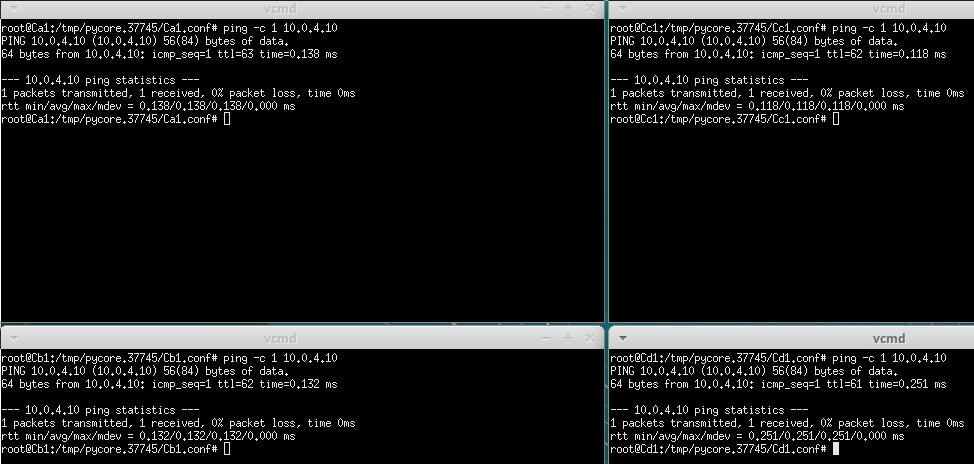
\includegraphics[width=\textwidth]{images/pingEx1P2.png}
    \caption{Ex.1 - Ping}
    \label{fig:pingEx1P2}
\end{figure}

\pagebreak
\section{Exercício 2}

\begin{figure}[H]
    \centering 
    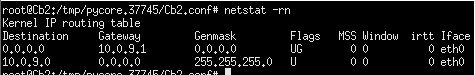
\includegraphics[width=\textwidth]{images/netstatPcEx2P2.png}
    \caption{Ex.2 - netstat pc departamento B}
    \label{fig:netstatPcEx2P2}
\end{figure}

\begin{figure}[H]
    \centering 
    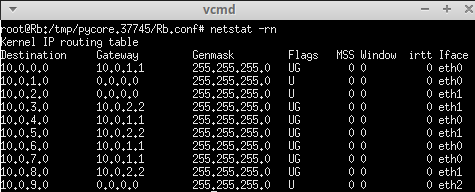
\includegraphics[width=\textwidth]{images/netstatRouterEx2P2.png}
    \caption{Ex.2 - netstat Router departamento B}
    \label{fig:netstatRouterEx2P2}
\end{figure}

\begin{figure}[H]
    \centering 
    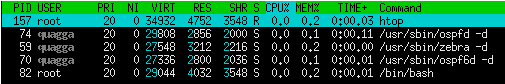
\includegraphics[width=\textwidth]{images/htop2a.png}
    \caption{Ex.2 - Processos a serem executados em Ra}
    \label{fig:htop2a}
\end{figure}

\begin{figure}[H]
    \centering 
    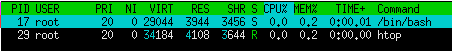
\includegraphics[width=\textwidth]{images/htopca1.png}
    \caption{Ex.2 - Processos a serem executados em Ca1}
    \label{fig:htopca1}
\end{figure}

\pagebreak
\section{Exercício 3}

\end{document}
